\documentclass[10pt]{beamer}
\usetheme[
%%% options passed to the outer theme
%    progressstyle=movCircCnt,   %either fixedCircCnt, movCircCnt, or corner
%    rotationcw,          % change the rotation direction from counter-clockwise to clockwise
%    shownavsym          % show the navigation symbols
  ]{AAUsimple}

% If you want to change the colors of the various elements in the theme, edit and uncomment the following lines
% Change the bar and sidebar colors:
%\setbeamercolor{AAUsimple}{fg=red!20,bg=red}
%\setbeamercolor{sidebar}{bg=red!20}
% Change the color of the structural elements:
%\setbeamercolor{structure}{fg=red}
% Change the frame title text color:
%\setbeamercolor{frametitle}{fg=blue}
% Change the normal text color background:
%\setbeamercolor{normal text}{fg=black,bg=gray!10}
% ... and you can of course change a lot more - see the beamer user manual.

% 
\usepackage{stmaryrd}

\usepackage{listings}
% default style
\lstdefinestyle{default}{
  numbers=left,
  frame=single,
  captionpos=b,
  backgroundcolor=\color{cyan!10},
  showstringspaces=false,
  breaklines=true
}
% python style
\lstdefinestyle{python}{
  style=default,
  language=Python,
  basicstyle=\small\tt,
  keywordstyle=\color{blue},
  commentstyle=\color[rgb]{0.13,0.54,0.13},
  backgroundcolor=\color{cyan!10},
  morekeywords={
    True,
    False
  },
  deletendkeywords={filter, all, file, format}
}
\usepackage{color}

\usepackage[utf8]{inputenc}
\usepackage[english]{babel}
\usepackage[T1]{fontenc}

\usepackage{pgf}
\usepackage{tikz}
\usepackage{marvosym}
\usetikzlibrary{positioning}
\usetikzlibrary{shapes}
\usetikzlibrary{arrows.meta}
\usetikzlibrary{arrows,automata}

\usepackage{graphicx}
\graphicspath{{/graphics/}}
\usepackage{tikzscale}
\usepackage{subcaption}
\captionsetup{compatibility=false}

% Or whatever. Note that the encoding and the font should match. If T1
% does not look nice, try deleting the line with the fontenc.
\usepackage{helvet}
\usepackage{comment}

% colored hyperlinks
\newcommand{\chref}[2]{%
  \href{#1}{{\usebeamercolor[bg]{AAUsimple}#2}}%
}

\newcommand{\constraint}[1]{
\llbracket #1 \rrbracket
  }

\newcommand{\assignconstraint}[1]{
\llbracket {\color{red}#1} \rrbracket
}

\title{PyT}

%\subtitle{Any suggestions for subtitle?}  % could also be a conference name

\date{\today}

\author[B. Thalmann, S. Micheelsen]{
  Bruno Thalmann\\
  Stefan Marstrand Getreuer Micheelsen\\
}

% - Give the names in the same order as they appear in the paper.
% - Use the \inst{?} command only if the authors have different
%   affiliation. See the beamer manual for an example

\institute[
%  {\includegraphics[scale=0.2]{aau_segl}}\\ %insert a company, department or university logo
  Dept.\ of Computer Science\\
  Aalborg University\\
  Denmark
] % optional - is placed in the bottom of the sidebar on every slide
{% is placed on the title page
  Department of Computer Science\\
  Aalborg University\\
  Denmark

  %there must be an empty line above this line - otherwise some unwanted space is added between the university and the country (I do not know why;( )
}

% specify a logo on the titlepage (you can specify additional logos an include them in
% institute command below
\pgfdeclareimage[height=1.5cm]{titlepagelogo}{AAUgraphics/aau_logo_new} % placed on the title page
%\pgfdeclareimage[height=1.5cm]{titlepagelogo2}{AAUgraphics/aau_logo_new} % placed on the title page
\titlegraphic{% is placed on the bottom of the title page
  \pgfuseimage{titlepagelogo}
%  \hspace{1cm}\pgfuseimage{titlepagelogo2}
}

\begin{document}
% the titlepage
{\aauwavesbg%
\begin{frame}[plain,noframenumbering] % the plain option removes the header from the title page
  \titlepage
\end{frame}}
%%%%%%%%%%%%%%%%

% CONTENT
\begin{frame}
  \begin{tikzpicture}[remember picture,overlay]
    \fill [white] (current page.south west) rectangle (current page.north east);
    \node at (current page.center) {\resizebox{!}{\textheight}{ \begin{tikzpicture}
\newcommand\XLabel{7}
\newcommand\XNode{10}
\newcommand\XEngines{14}
\newcommand\TextWidth{3}
\tikzset{>=latex}

%\draw[help lines] (5,5) grid (15,20);

%%%%%%%%%%%% MID STRUCTURE %%%%%%%%%%%%%%%%%%%
\node[inner sep=10pt] (code) at (\XNode,18)
    {
\includegraphics[width=.1\textwidth]{./graphics/implementation_overview_images/source_code.png}};
\node[text width=\TextWidth{}cm] at (\XLabel,18) {\hfill{}Source code};

\node[inner sep=10pt] (ast) at (\XNode,15)
    {
\includegraphics[width=.15\textwidth]{./graphics/implementation_overview_images/ast.png}};
\node[text width=\TextWidth{}cm] at (\XLabel,15) {\hfill{}AST};

\node[inner sep=10pt] (cfg) at (\XNode,11)
    {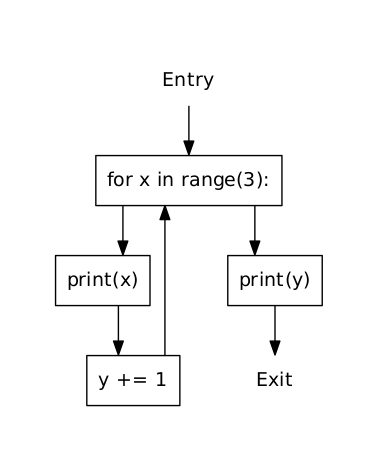
\includegraphics[width=.2\textwidth]{./graphics/implementation_overview_images/for_complete.png}};
\node[text width=\TextWidth{}cm] at (\XLabel,11) {\hfill{}CFG};

\node[inner sep=10pt] (engine) at (\XNode,7)
    {
\includegraphics[width=.1\textwidth]{./graphics/implementation_overview_images/cog_wheel.png}};
\node[text width=\TextWidth{}cm] at (\XLabel,7) {\hfill{}Framework \\ \hfill{}Adaptor};

\node[inner sep=10pt] (algorithm) at (\XNode,4)
    {
\includegraphics[width=.1\textwidth]{./graphics/implementation_overview_images/spiral.png}};
\node[text width=\TextWidth{}cm] at (\XLabel,4) {\hfill{}Fixed Point \\ \hfill{}Algorithm};

\node[inner sep=10pt] (vulnerabilities) at (\XNode,1)
    {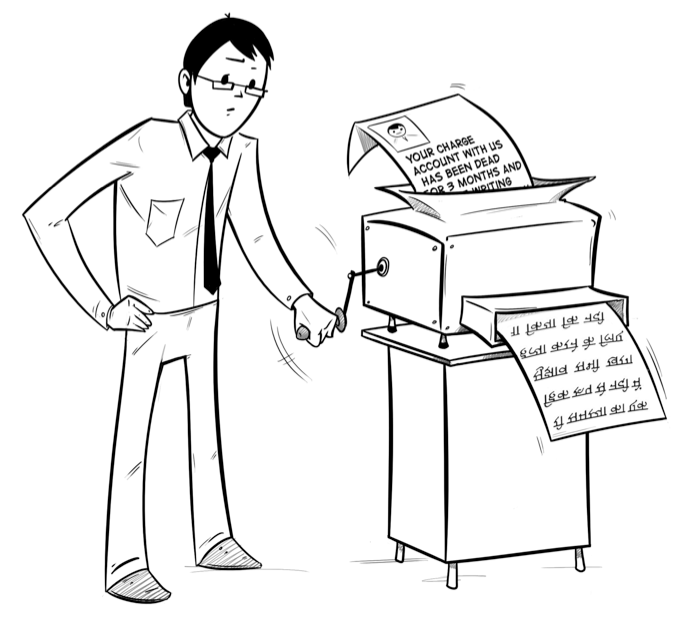
\includegraphics[width=.15\textwidth]{./graphics/implementation_overview_images/vulnerability.png}};
\node[text width=\TextWidth{}cm] at (\XLabel,1) {\hfill{}Vulnerabilities};

%%%%%%%%%%%%%%%%%%%% Adaptors %%%%%%%%%%%%%%%%%%%%%%%%
\node[inner sep=10pt] (flask) at (\XEngines,11)
    {
\includegraphics[width=.2\textwidth]{./graphics/implementation_overview_images/flask_text.png}};

\node[inner sep=5pt] (django) at (\XEngines,9)
    {
\includegraphics[width=.13\textwidth]{./graphics/implementation_overview_images/django.png}};

\node[label=below:{Other}, inner sep=5pt] (other_engine) at (\XEngines,7)
    {
\includegraphics[width=.05\textwidth]{./graphics/implementation_overview_images/question_mark.png}};

%%%%%%%%%%%%%%%% ANALYSIS %%%%%%%%%%%%%%%%%%%%%%%%%    
\node[label=below:{Analysis}, inner sep=10pt] (analysis) at (\XEngines,4)
    {
\includegraphics[width=.1\textwidth]{./graphics/implementation_overview_images/analysis.png}};

\node[text width=2cm, inner sep=10pt] (reaching) at (18,7) {Reaching Definitions};
\node[text width=2cm, inner sep=10pt] (liveness) at (18,4) {Liveness};

\node[label=below:{Other}, inner sep=5pt] (other_analysis) at (18,1)
    {
\includegraphics[width=.05\textwidth]{./graphics/implementation_overview_images/question_mark.png}};


\draw[->] (code) -- (ast);
\draw[->] (ast) -- (cfg);
\draw[->] (cfg) -- (engine);
\draw[->] (engine) -- (algorithm);
\draw[->] (algorithm) -- (vulnerabilities);

\draw[->] (flask) -- (engine);
\draw[->] (django) -- (engine);
\draw[->] (other_engine) -- (engine);

\draw[<->] (algorithm) -- (analysis);
\draw[->] (reaching) -- (analysis);
\draw[->] (liveness) -- (analysis);
\draw[->] (other_analysis) -- (analysis);

\end{tikzpicture}}};
  \end{tikzpicture}
\end{frame}

\begin{frame}[plain]
  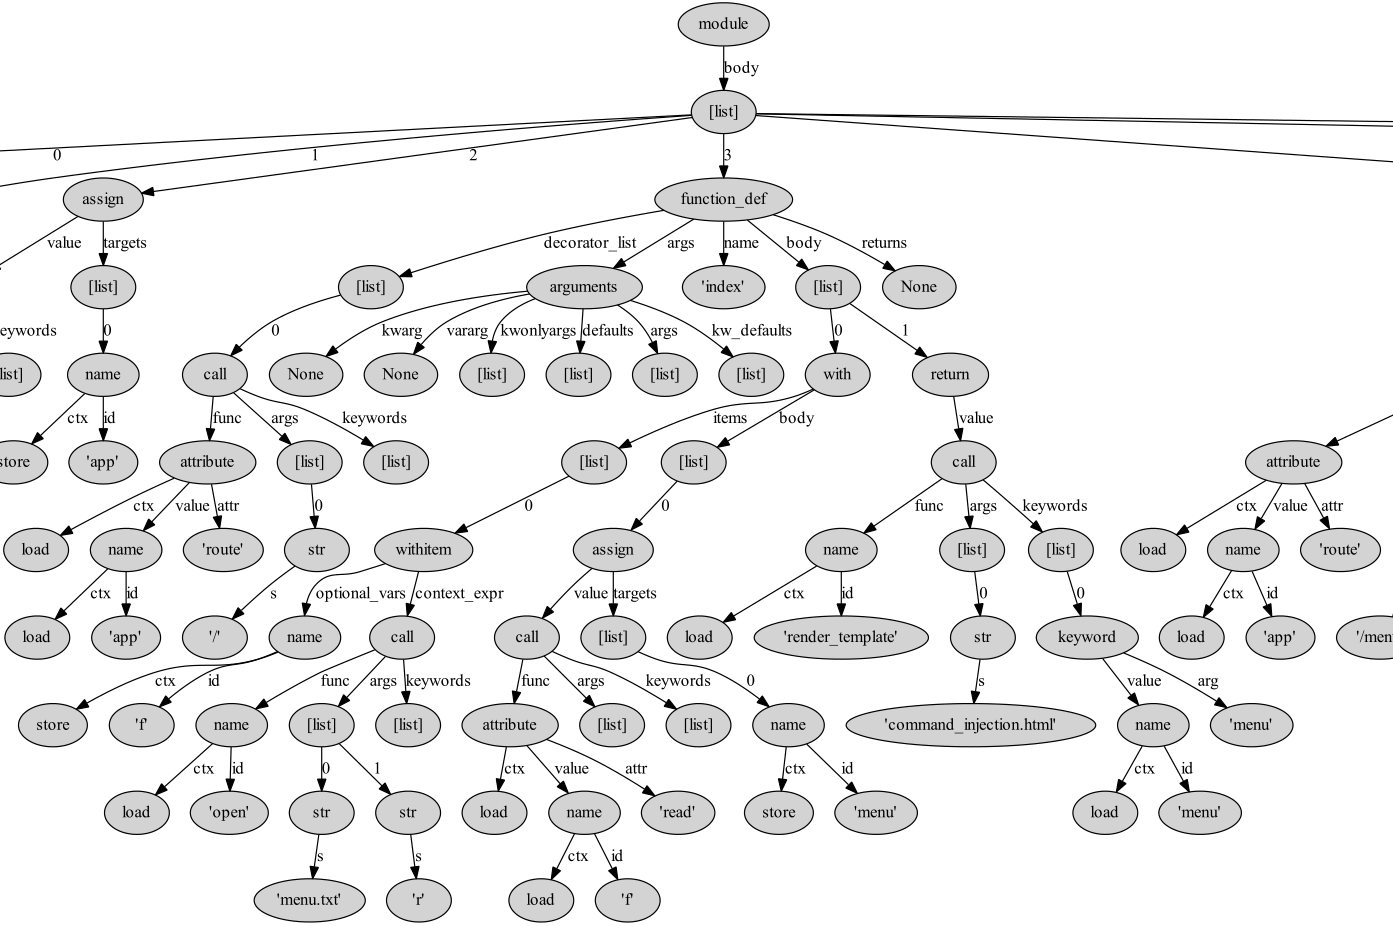
\includegraphics[width=\textwidth]{graphics/AST}
\end{frame}

\begin{frame}[fragile, plain]
  \begin{lstlisting}[style=default]
mod = Module(stmt* body)

stmt = FunctionDef(identifier name, arguments args, stmt* body, expr* decorator_list, expr? returns)
     | Assign(expr* targets, expr value)
     | With(withitem* items, stmt* body)
     | Return(expr? value)
       
expr = Call(expr func, expr* args, keyword* keywords)
     | Attribute(expr value, identifier attr, expr_context ctx)
     | Num(object n)
     | Name(identifier id, expr_context ctx)
     | Str(string s)   
  \end{lstlisting}
\end{frame}

\begin{frame}
  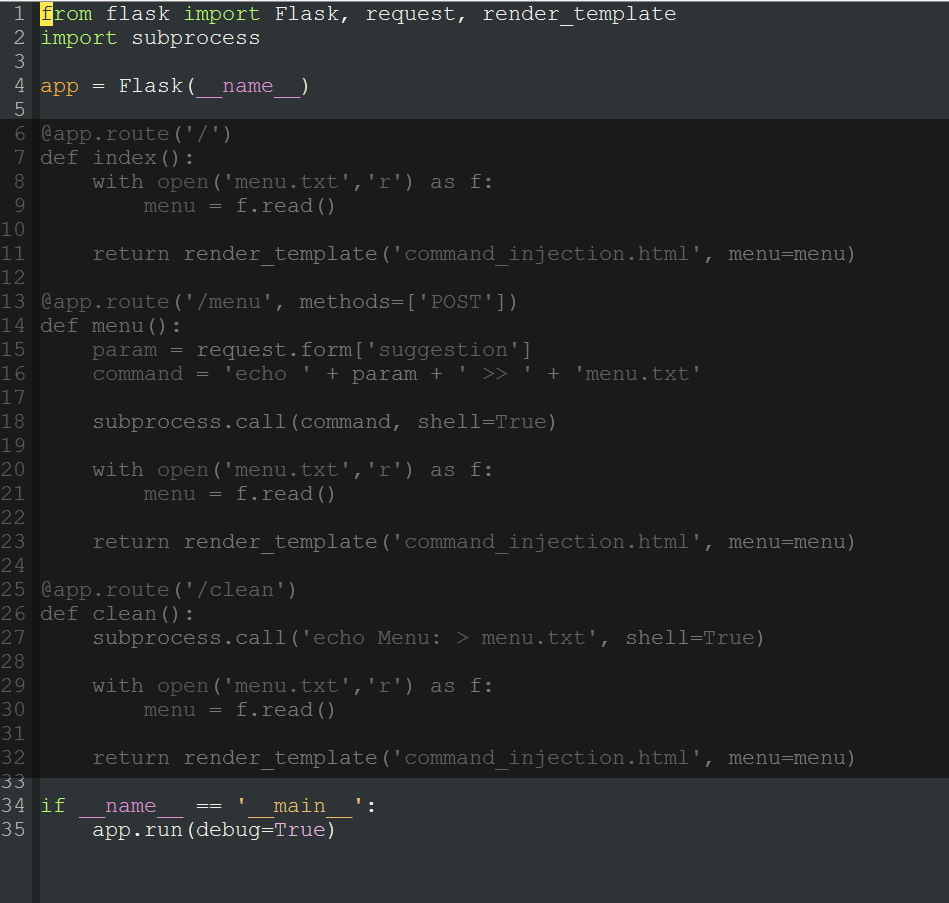
\includegraphics[height=0.8\textheight]{graphics/adaptor_module}
\end{frame}


\begin{frame}{Control Flow Graphs}
    \center
    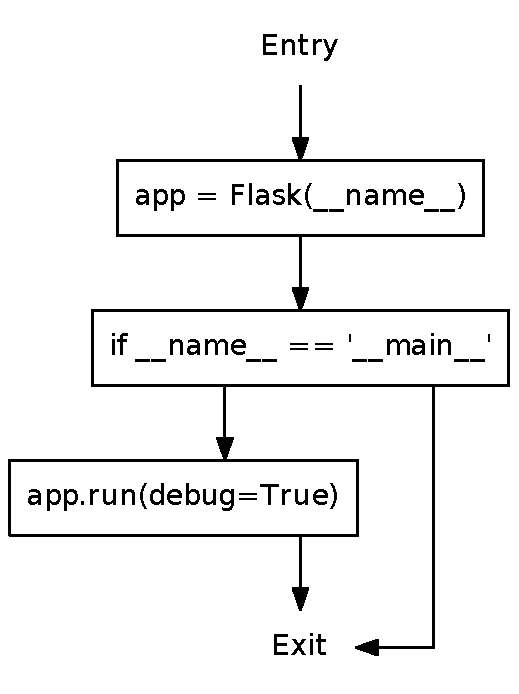
\includegraphics[height=0.8\textheight]{graphics/CFG_module}
\end{frame}

\begin{frame}
  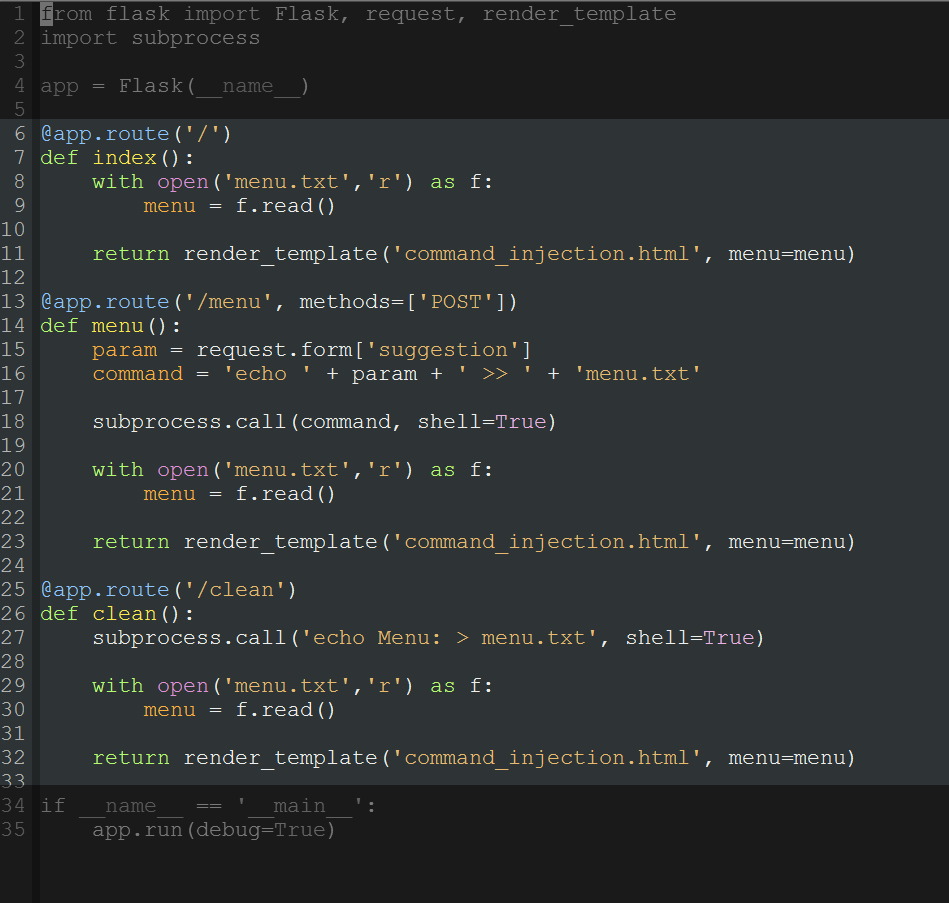
\includegraphics[height=0.8\textheight]{graphics/adaptor_flask}
\end{frame}


\begin{frame}{Control Flow Graphs}
  \center
  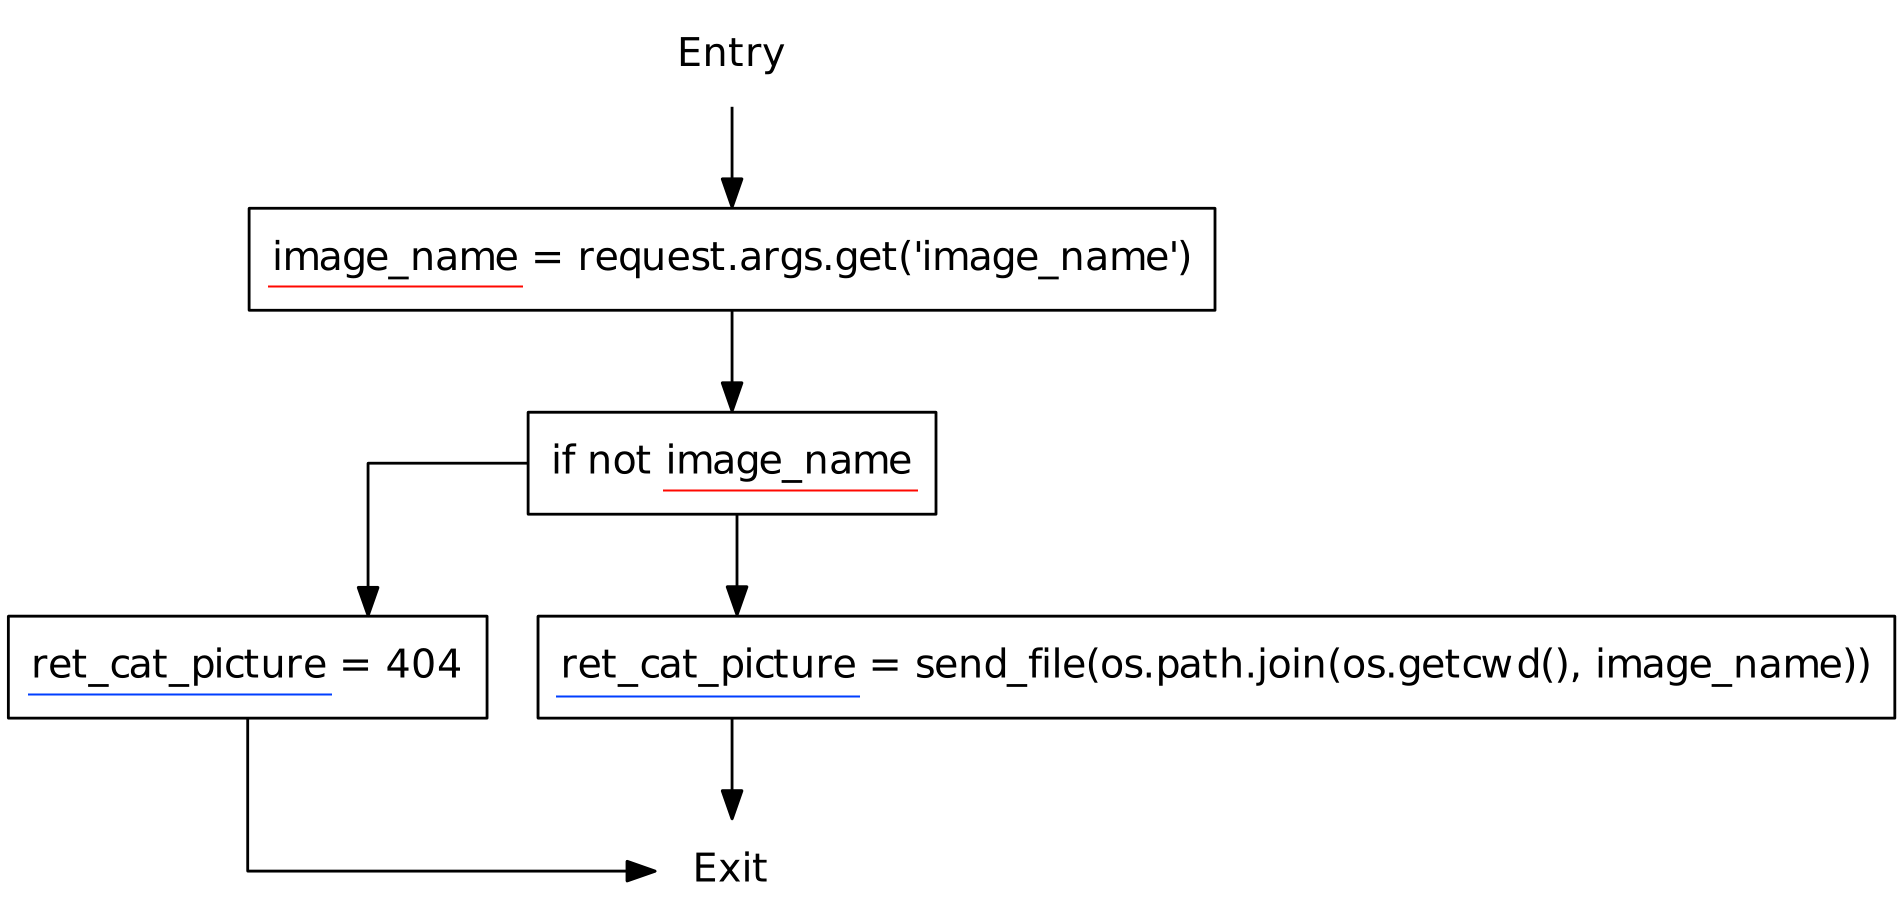
\includegraphics[height=0.75\textheight]{graphics/cfg_path_traversal}
\end{frame}



\begin{frame}
  \center
  
\includegraphics[width=\textwidth]{graphics/adaptor}
\end{frame}

\begin{frame}
  \begin{tikzpicture}[remember picture,overlay]
    \fill [white] (current page.south west) rectangle (current page.north east);
    \node at (current page.center) {\resizebox{!}{\textheight}{ \begin{tikzpicture}
\newcommand\XLabel{7}
\newcommand\XNode{10}
\newcommand\XEngines{14}
\newcommand\TextWidth{3}
\tikzset{>=latex}

%\draw[help lines] (5,5) grid (15,20);

%%%%%%%%%%%% MID STRUCTURE %%%%%%%%%%%%%%%%%%%
\node[inner sep=10pt] (code) at (\XNode,18)
    {
\includegraphics[width=.1\textwidth]{./graphics/implementation_overview_images/source_code.png}};
\node[text width=\TextWidth{}cm] at (\XLabel,18) {\hfill{}Source code};

\node[inner sep=10pt] (ast) at (\XNode,15)
    {
\includegraphics[width=.15\textwidth]{./graphics/implementation_overview_images/ast.png}};
\node[text width=\TextWidth{}cm] at (\XLabel,15) {\hfill{}AST};

\node[inner sep=10pt] (cfg) at (\XNode,11)
    {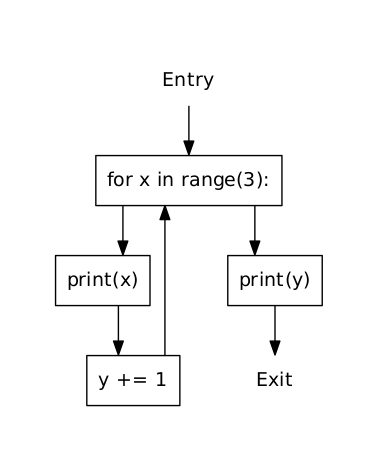
\includegraphics[width=.2\textwidth]{./graphics/implementation_overview_images/for_complete.png}};
\node[text width=\TextWidth{}cm] at (\XLabel,11) {\hfill{}CFG};

\node[inner sep=10pt] (engine) at (\XNode,7)
    {
\includegraphics[width=.1\textwidth]{./graphics/implementation_overview_images/cog_wheel.png}};
\node[text width=\TextWidth{}cm] at (\XLabel,7) {\hfill{}Framework \\ \hfill{}Adaptor};

\node[inner sep=10pt] (algorithm) at (\XNode,4)
    {
\includegraphics[width=.1\textwidth]{./graphics/implementation_overview_images/spiral.png}};
\node[text width=\TextWidth{}cm] at (\XLabel,4) {\hfill{}Fixed Point \\ \hfill{}Algorithm};
\draw[red, very thick] (\XNode-1, 4) ellipse (3cm and 1.25cm);

\node[inner sep=10pt] (vulnerabilities) at (\XNode,1)
    {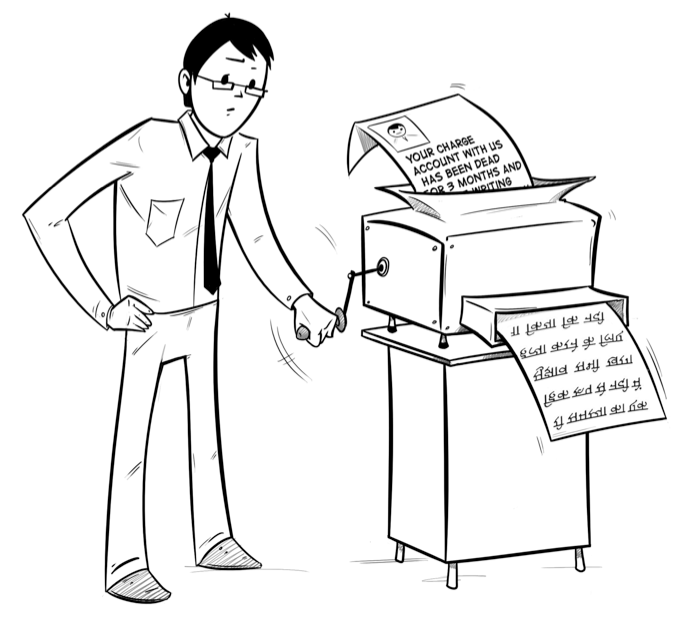
\includegraphics[width=.15\textwidth]{./graphics/implementation_overview_images/vulnerability.png}};
\node[text width=\TextWidth{}cm] at (\XLabel,1) {\hfill{}Vulnerabilities};

%%%%%%%%%%%%%%%%%%%% Adaptors %%%%%%%%%%%%%%%%%%%%%%%%
\node[inner sep=10pt] (flask) at (\XEngines,11)
    {
\includegraphics[width=.2\textwidth]{./graphics/implementation_overview_images/flask_text.png}};

\node[inner sep=5pt] (django) at (\XEngines,9)
    {
\includegraphics[width=.13\textwidth]{./graphics/implementation_overview_images/django.png}};

\node[label=below:{Other}, inner sep=5pt] (other_engine) at (\XEngines,7)
    {
\includegraphics[width=.05\textwidth]{./graphics/implementation_overview_images/question_mark.png}};

%%%%%%%%%%%%%%%% ANALYSIS %%%%%%%%%%%%%%%%%%%%%%%%%    
\node[label=below:{Analysis}, inner sep=10pt] (analysis) at (\XEngines,4)
    {
\includegraphics[width=.1\textwidth]{./graphics/implementation_overview_images/analysis.png}};

\node[text width=2cm, inner sep=10pt] (reaching) at (18,7) {Reaching Definitions};
\node[text width=2cm, inner sep=10pt] (liveness) at (18,4) {Liveness};

\node[label=below:{Other}, inner sep=5pt] (other_analysis) at (18,1)
    {
\includegraphics[width=.05\textwidth]{./graphics/implementation_overview_images/question_mark.png}};


\draw[->] (code) -- (ast);
\draw[->] (ast) -- (cfg);
\draw[->] (cfg) -- (engine);
\draw[->] (engine) -- (algorithm);
\draw[->] (algorithm) -- (vulnerabilities);

\draw[->] (flask) -- (engine);
\draw[->] (django) -- (engine);
\draw[->] (other_engine) -- (engine);

\draw[<->] (algorithm) -- (analysis);
\draw[->] (reaching) -- (analysis);
\draw[->] (liveness) -- (analysis);
\draw[->] (other_analysis) -- (analysis);

\end{tikzpicture}}};
  \end{tikzpicture}
\end{frame}

\begin{frame}{Lattice}
  \begin{itemize}
  \item Partial order 
  \item Least upper bound for all subsets
  \item Greatest lower bound for all subsets
  \end{itemize}


  \begin{figure}
    \begin{subfigure}[b]{0.4\textwidth}
      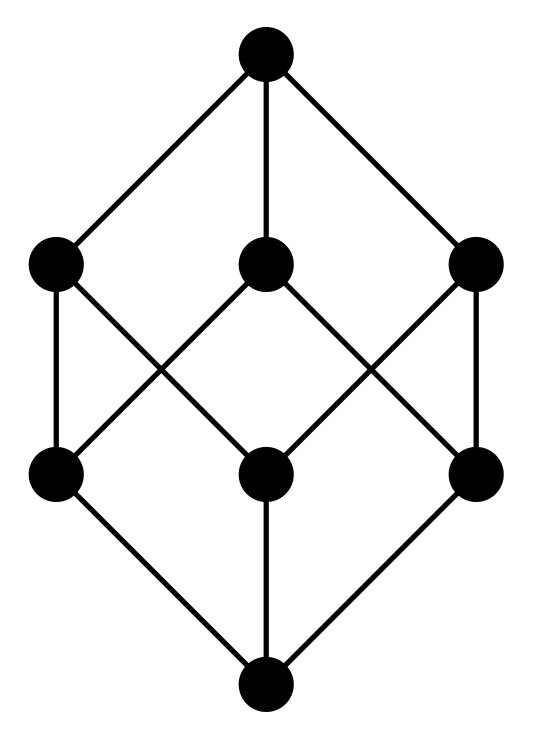
\includegraphics[width=0.6\textwidth]{graphics/lattice}
    \end{subfigure}
    ~
    \begin{subfigure}[b]{0.4\textwidth}
      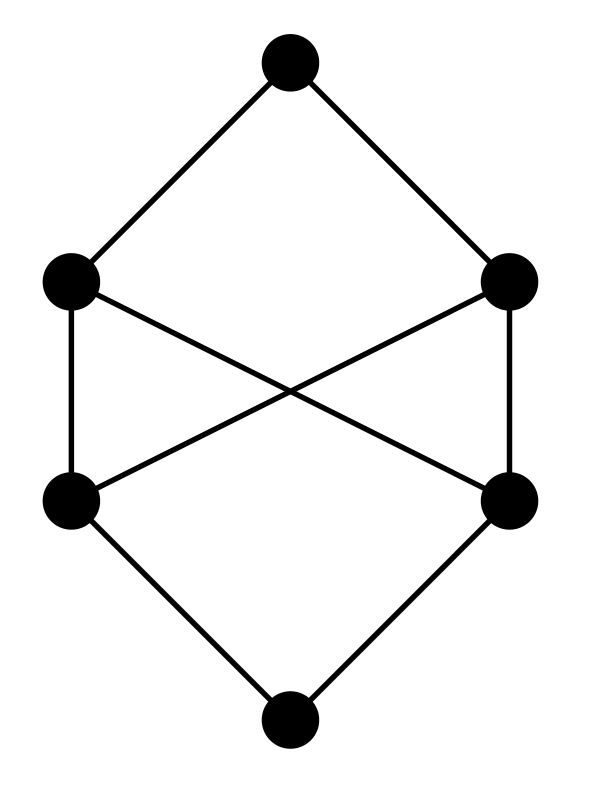
\includegraphics[width=0.6\textwidth]{graphics/notlattice}
    \end{subfigure}    
  \end{figure}
\end{frame}

\begin{frame}{Lattice}
  \begin{itemize}
  \item Partial order 
  \item Least upper bound for all subsets
  \item Greatest lower bound for all subsets
  \end{itemize}


  \begin{figure}
    \begin{subfigure}[b]{0.4\textwidth}
      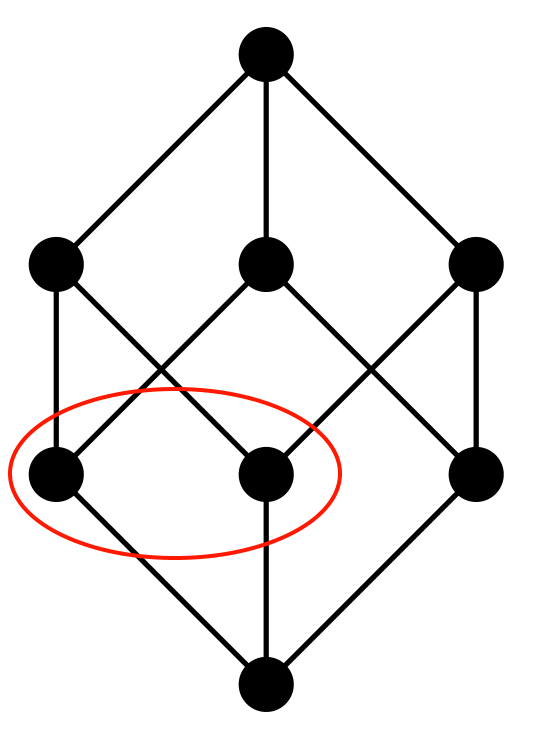
\includegraphics[width=0.6\textwidth]{graphics/lattice_low}
    \end{subfigure}
    ~
    \begin{subfigure}[b]{0.4\textwidth}
      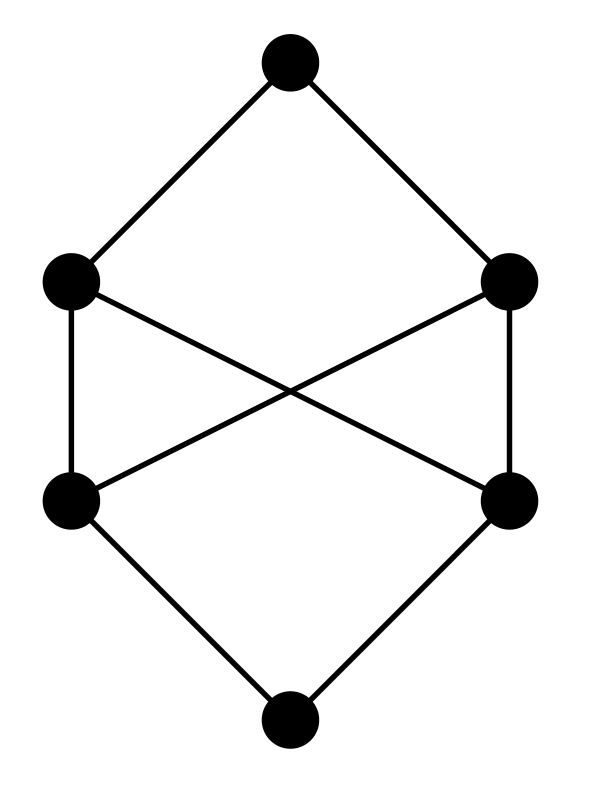
\includegraphics[width=0.6\textwidth]{graphics/notlattice}
    \end{subfigure}    
  \end{figure}
\end{frame}

\begin{frame}{Lattice}
  \begin{itemize}
  \item Partial order 
  \item Least upper bound for all subsets
  \item Greatest lower bound for all subsets
  \end{itemize}


  \begin{figure}
    \begin{subfigure}[b]{0.4\textwidth}
      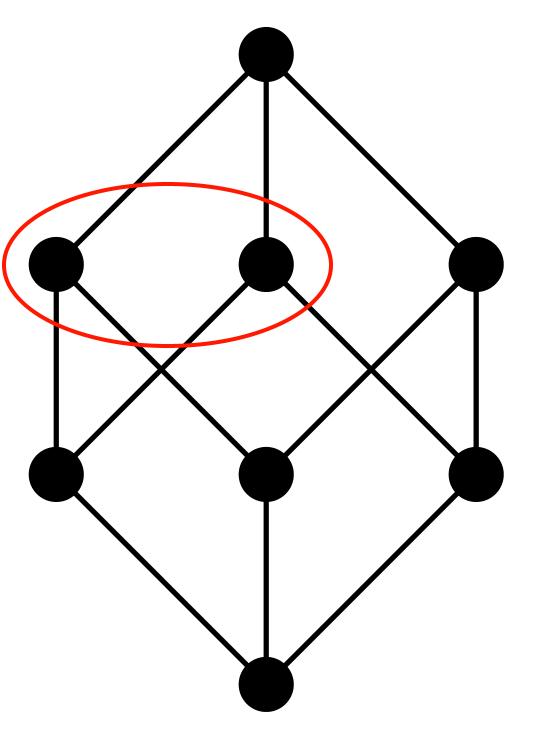
\includegraphics[width=0.6\textwidth]{graphics/lattice_high}
    \end{subfigure}
    ~
    \begin{subfigure}[b]{0.4\textwidth}
      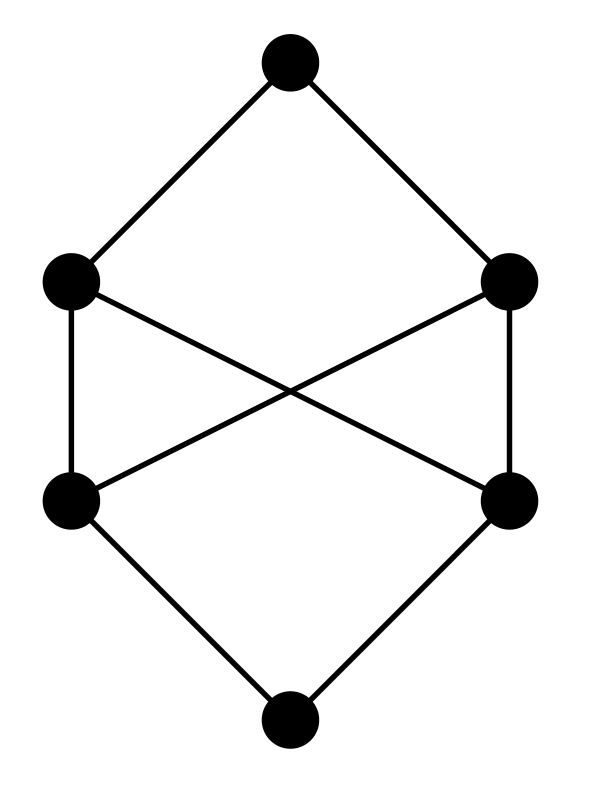
\includegraphics[width=0.6\textwidth]{graphics/notlattice}
    \end{subfigure}    
  \end{figure}
\end{frame}

\begin{frame}{Lattice}
  \begin{itemize}
  \item Partial order 
  \item Least upper bound for all subsets
  \item Greatest lower bound for all subsets
  \end{itemize}


  \begin{figure}
    \begin{subfigure}[b]{0.4\textwidth}
      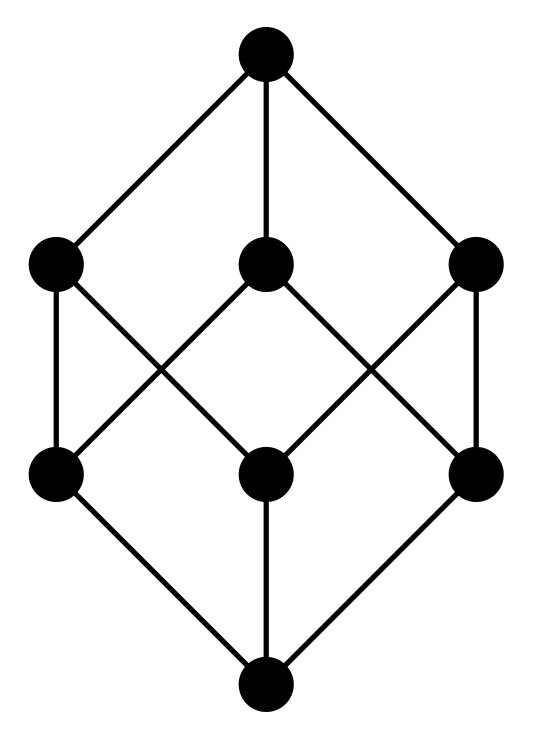
\includegraphics[width=0.6\textwidth]{graphics/lattice}
    \end{subfigure}
    ~
    \begin{subfigure}[b]{0.4\textwidth}
      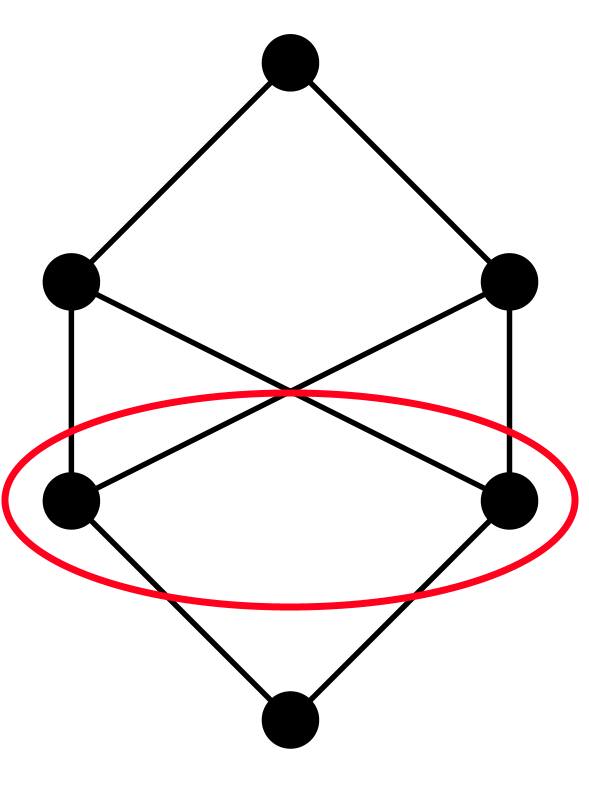
\includegraphics[width=0.6\textwidth]{graphics/notlatticepoints}
    \end{subfigure}    
  \end{figure}
\end{frame}

\begin{frame}{Lattice}
  \begin{itemize}
  \item Partial order 
  \item Least upper bound for all subsets
  \item Greatest lower bound for all subsets
  \end{itemize}


  \begin{figure}
    \begin{subfigure}[b]{0.4\textwidth}
      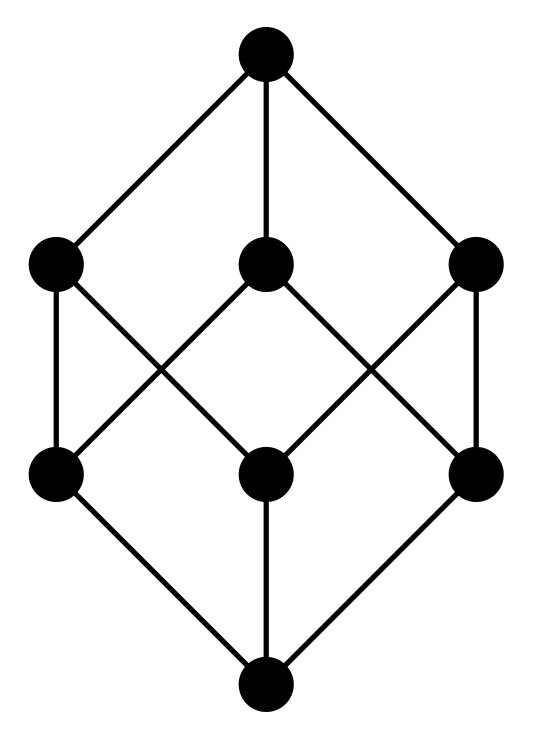
\includegraphics[width=0.6\textwidth]{graphics/lattice}
    \end{subfigure}
    ~
    \begin{subfigure}[b]{0.4\textwidth}
      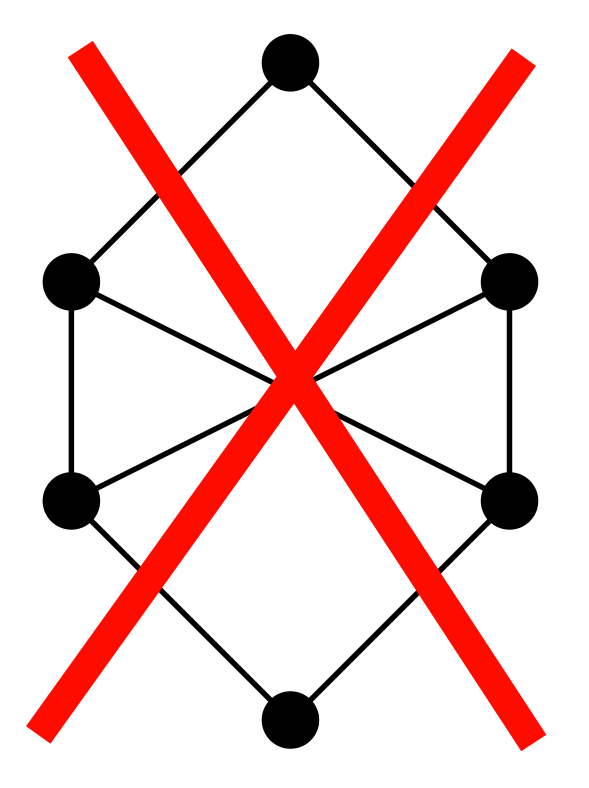
\includegraphics[width=0.6\textwidth]{graphics/definitelynotlattice}
    \end{subfigure}    
  \end{figure}
\end{frame}

\newcommand{\constraint}[1]{
\llbracket #1 \rrbracket
  }

\newcommand{\assignconstraint}[1]{
\llbracket {\color{red}#1} \rrbracket
  }




\begin{frame}
\[
\begin{array}{lclcl}
  \constraint{entry} & = & \{\} &\phantom{hahahahhh}\\
  \assignconstraint{param} & = & \{\} &\\
  \assignconstraint{command} & = & \{\}&\\
  \constraint{subprocess.call} & = & \{\}&\\
  \constraint{with} & = & \{\}&\\
  \assignconstraint{menu} & = & \{\}&\\
  \assignconstraint{ret\_f.read} & = & \{\}&\\
  \constraint{exit} & = & \{\}&\\
  && \phantom{\{command, param\}} && \phantom{\{command, param\}}
\end{array}
\]
\end{frame}

\begin{frame}
\[
\begin{array}{lclcl}
  \constraint{entry} & = & \{\} & \rightarrow & \{\}\\
  \assignconstraint{param} & = & \{\} & \rightarrow &\{param\}\\
  \assignconstraint{command} & = & \{\}& \rightarrow &\{command\}\\
  \constraint{subprocess.call} & = & \{\}& \rightarrow &\{\}\\
  \constraint{with} & = & \{\}&\rightarrow & \{\}\\
  \assignconstraint{menu} & = & \{\}& \rightarrow & \{menu\}\\
  \assignconstraint{ret\_f.read} & = & \{\}&\rightarrow & \{ret\_f.read\}\\
  \constraint{exit} & = & \{\}&\rightarrow & \{\}\\
  && && \phantom{\{command, param\}\{command, param\}}
\end{array}
\]
\end{frame}

\begin{frame}
\[
\begin{array}{lclcl}
  \constraint{entry} & = &  \{\} & \phantom{\rightarrow} & \phantom{hahahaha}\\
  \assignconstraint{param} & = & \{param\}&  & \\ 
  \assignconstraint{command} & = &\{command\}&  & \\
  \constraint{subprocess.call} & = & \{\}&  & \\
  \constraint{with} & = & \{\}&  & \\
  \assignconstraint{menu} & = &  \{menu\}&  & \\
  \assignconstraint{ret\_f.read} & = & \{ret\_f.read\}&  & \\
  \constraint{exit} & = & \{\}&  & \\
  && && \phantom{\{command, param\} \{command, param\}}
\end{array}
\]
\end{frame}

\begin{frame}
  \[
\begin{array}{lclcl}
  \constraint{entry} & = &  \{\} & \rightarrow & \{\}\\
  \assignconstraint{param} & = & \{param\}& \rightarrow & \{param\}\\ 
  \assignconstraint{command} & = &\{command\}& \rightarrow & \{command, param\}\\
  \constraint{subprocess.call} & = & \{\}& \rightarrow & \{command\}\\
  \constraint{with} & = & \{\}& \rightarrow & \{\}\\
  \assignconstraint{menu} & = &  \{menu \}& \rightarrow & \{menu\} \\
  \assignconstraint{ret\_f.read} & = & \{ret\_f.read\}& \rightarrow & \{ret\_f.read, menu\}\\
  \constraint{exit} & = & \{\}& \rightarrow & \{ret\_f.read\}\\
  && && \phantom{\{command, param\}\{command, param\}}
\end{array}
\]
\end{frame}


\begin{frame}
  \[
\begin{array}{lclcl}
  \constraint{entry} & = & \{\}& \phantom{\rightarrow} & \phantom{\{command, param\}} \\
  \assignconstraint{param} & = & \{param\}& \\ 
  \assignconstraint{command} & = & \{command, param\}& \\
  \constraint{subprocess.call} & = & \{command\}& \\
  \constraint{with} & = & \{\}& \\
  \assignconstraint{menu} & = & \{menu\} & \\
  \assignconstraint{ret\_f.read} & = & \{ret\_f.read, menu\}& \\
  \constraint{exit} & = & \{ret\_f.read\}& \\
  && \phantom{\{command, param\}} && \phantom{\{command, param\}}
\end{array}
\]
\end{frame}


\begin{frame}
  \[
\begin{array}{lclcl}
  \constraint{entry} & = & \{\}& \rightarrow & \{\} \\
  \assignconstraint{param} & = & \{param\}& \rightarrow & \{param\}\\ 
  \assignconstraint{command} & = & \{command , param \}& \rightarrow & \{command, param\}\\
  \constraint{subprocess.call} & = & \{command\}& \rightarrow & \{command, param\}\\
  \constraint{with} & = & \{\}& \rightarrow & \{command\}\\
  \assignconstraint{menu} & = & \{menu\} & \rightarrow & \{menu\}\\
  \assignconstraint{ret\_f.read} & = & \{ret\_f.read, menu\}& \rightarrow & \{ret_f.read, menu\}\\
  \constraint{exit} & = & \{ret\_f.read\}& \rightarrow & \{ret_f.read, menu\}\\
  && && \phantom{\{command, param\}}
\end{array}
\]
\end{frame}

\begin{frame}
  \[
\begin{array}{lclcl}
  \constraint{entry} & = & \{command, param\} & \phantom{\rightarrow} & \phantom{\{command, param\}}\\
  \assignconstraint{param} & = & \{param\} \\ 
  \assignconstraint{command} & = & \{command, param\}\\
  \constraint{subprocess.call} & = & \{command, param\}\\
  \constraint{with} & = & \{command\} \\
  \assignconstraint{menu} & = & \{menu\}\\
  \assignconstraint{ret\_f.read} & = & \{ret_f.read, menu\}\\
  \constraint{exit} & = & \{ret_f.read, menu\}\\
  &&  && \phantom{\{command, param\}}
\end{array}
\]
\end{frame}

\begin{frame}
  \[
\begin{array}{lclcl}
  \constraint{entry} & = & \dots & \rightarrow & {\{\}}\\
  \assignconstraint{param} & = & \dots & \rightarrow & \{param\} \\ 
  \assignconstraint{command} & = & \dots & \rightarrow & \{command, param\}\\
  \constraint{subprocess.call} & = & \dots & \rightarrow & \{command, param\}\\
  \constraint{with} & = & \dots & \rightarrow & \{command, param\} \\
  \assignconstraint{menu} & = & \dots & \rightarrow & \{menu, command, param\}\\
  \assignconstraint{ret\_f.read} & = & \dots & \rightarrow & \{ret_f.read, menu, command, param\}\\
  \constraint{exit} & = & \dots & \rightarrow & \{ret_f.read, menu, command, param\}\\
  &&&&
\end{array}
\]
\end{frame}

% the final page
{\aauwavesbg
\begin{frame}[plain,noframenumbering]
  \finalpage{Thank you for your time}
\end{frame}}

\end{document}
